\section{Performance}
\subsection{Improvements}

To establish the performance of the final code, we made a comparison in Table \ref{table:table1}, using the first day data as a baseline. In the baseline code, that is our solution developed for the first assignment, buses only travel around all bus stops, pick up passengers and drop off them. In the final version, we implemented all the improvements explained in Section \ref{sec:conceptual}.

\begin{table*}[htbp]
\centering
\begin{tabular}{ |c|c|c|  }
 \hline
  Measurement & Baseline & Final Code \\
 \hline
  Avg travel time & 150 & 72.53 \\
  Buses' expenses & 1039682 & 711251 \\
  Messages sent & 0 & 285  \\
  Final amount waiting & 232 & 255 \\
  Avg travel time remaining & 100 & 78.12 \\
  Final avg travel time & 156 & 75.48 \\
 \hline
\end{tabular}
\label{table:table1}
\caption{Performance results}
\end{table*}

Table \ref{table:table1} shows that there is a significant decrease in the average traveling times and costs. Obviously, the number of messages increase because during the first version no message was sent. However, the number of people waiting at the end of the simulation slightly increases in the newer version.

This result highlights the advantages of an intelligent coordination and competition between buses compared to a system of buses that does not exploit these concepts.

\subsection{Performance on test data}

For this project, we have three different data set, corresponding to three different days. We used day 1 to improve our solution, while day 4 and 5 as tests for our proposal. In this section, we show the results of our solution in the three different data sets.

The final value of the different metrics for the dataset of Day 1 are shown in the right column of Table \ref{table:table1}, whereas the plots for the expenses, the messages, the number of people waiting and the travelling time are shown in Figure \ref{fig:expense}, \ref{fig:messages}, \ref{fig:pass_waiting} and \ref{fig:avg_tt} respectively.

\begin{figure}[htbp]
\centering
\begin{minipage}{.48\textwidth}
  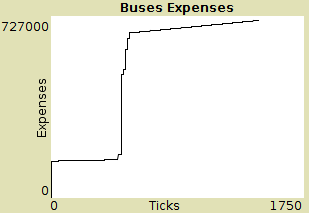
\includegraphics[width=\textwidth]{src/expenses.png}
  \caption{Expenses of the buses in Day 1.}
  \label{fig:expense}
\end{minipage}
\begin{minipage}{.48\textwidth}
  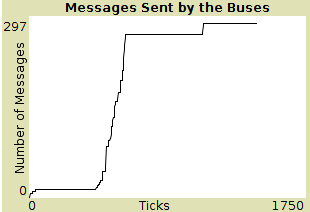
\includegraphics[width=\textwidth]{src/nr_messages.png}
  \caption{Number of exchanged messages in Day 1.}
  \label{fig:messages}
\end{minipage}
\end{figure}

\begin{figure}[htbp]
\centering
\begin{minipage}{.48\textwidth}
  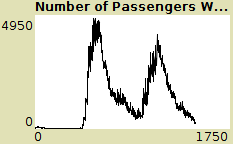
\includegraphics[width=\linewidth]{src/nr_pass_waiting.png}
  \caption{Final number of passengers waiting in Day 1.}
  \label{fig:pass_waiting}
\end{minipage}
\begin{minipage}{.48\textwidth}
  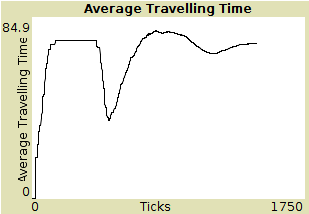
\includegraphics[width=\linewidth]{src/avg_tt.png}
  \caption{Average traveling time in Day 1.}
  \label{fig:avg_tt}
\end{minipage}
\end{figure}

Using the dataset of Day 1, we can see that there are two peeks in which the number of people suddenly appear in the map, and in which the fleet have to deal with this situation. It is important to note that during the first peek, our solution creates a number of buses that is probably enough to deal with the second peek (we can see a sudden increase in the bus expenses when there is the first peek, followed by a constant increase of the expenses for the rest of the simulation).

We are now going to focus on the results using the test sets, namely Day 4 and Day 5. In Table \ref{table:table2}, the metrics value on the two test sets are shown.

\begin{table*}[htbp]
\centering
\begin{tabular}{ |c|c|c|  }
 \hline
  Measurement & Test Data set 2 & Test Data set 3 \\
 \hline
  Avg travelling time & 92.36 & 86.72 \\
  Buses' expenses & 2393732 & 2346943.5 \\
  Messages sent & 950 & 992 \\
  Final amount waiting & 2603 & 2513 \\
  Avg travel time remaining & 182.97 & 206.91 \\
  Final avg travel time & 101.42 & 95.97 \\
 \hline
\end{tabular}
\label{table:table2}
\caption{Performance results}
\end{table*}

Our solution experienced a lot more difficulties in managing the situations of the test set. While the average travelling time is slighlty increased, compared to the one on the training set, we can notice a strong increase in the expenses and in the final amount of passengers waiting. 

The plots using Day 4 for the expenses, the messages, the number of people waiting and the travelling time are shown in Figure \ref{fig:expense4}, \ref{fig:messages4}, \ref{fig:pass_waiting4} and \ref{fig:avg_tt4} respectively.

\begin{figure}[htbp]
\centering
\begin{minipage}{.48\textwidth}
  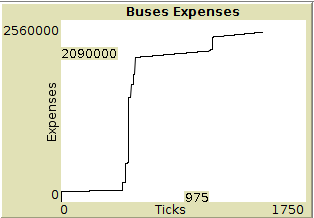
\includegraphics[width=\textwidth]{src/expenses4.png}
  \caption{Expenses of the buses in Day 4.}
  \label{fig:expense4}
\end{minipage}
\begin{minipage}{.48\textwidth}
  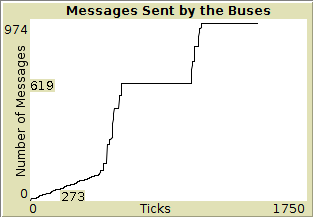
\includegraphics[width=\textwidth]{src/nr_messages4.png}
  \caption{Number of exchanged messages in Day 4.}
  \label{fig:messages4}
\end{minipage}
\end{figure}

\begin{figure}[htbp]
\centering
\begin{minipage}{.48\textwidth}
  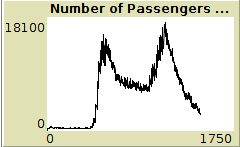
\includegraphics[width=\linewidth]{src/nr_pass_waiting4.png}
  \caption{Final number of passengers waiting in Day 4.}
  \label{fig:pass_waiting4}
\end{minipage}
\begin{minipage}{.48\textwidth}
  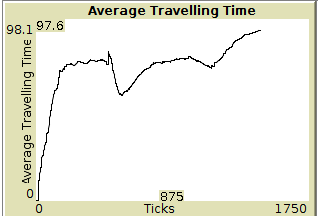
\includegraphics[width=\linewidth]{src/avg_tt4.png}
  \caption{Average travelling time in Day 4.}
  \label{fig:avg_tt4}
\end{minipage}
\end{figure}

The plots using Day 5 for the expenses, the messages, the number of people waiting and the travelling time are shown in Figure \ref{fig:expense5}, \ref{fig:messages5}, \ref{fig:pass_waiting5} and \ref{fig:avg_tt5} respectively.

\begin{figure}[htbp]
\centering
\begin{minipage}{.48\textwidth}
  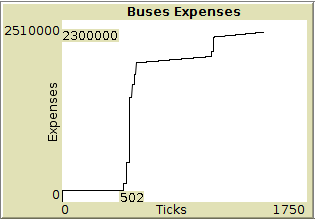
\includegraphics[width=\textwidth]{src/expenses5.png}
  \caption{Expenses of the buses in Day 5.}
  \label{fig:expense5}
\end{minipage}
\begin{minipage}{.48\textwidth}
  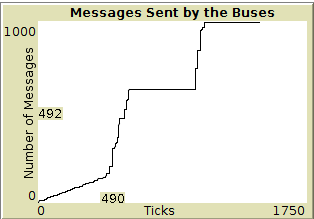
\includegraphics[width=\textwidth]{src/nr_messages5.png}
  \caption{Number of exchanged messages in Day 5.}
  \label{fig:messages5}
\end{minipage}
\end{figure}

\begin{figure}[htbp]
\centering
\begin{minipage}{.48\textwidth}
  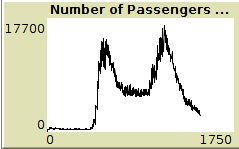
\includegraphics[width=\linewidth]{src/nr_pass_waiting5.png}
  \caption{Final number of passengers waiting in Day 5.}
  \label{fig:pass_waiting5}
\end{minipage}
\begin{minipage}{.48\textwidth}
  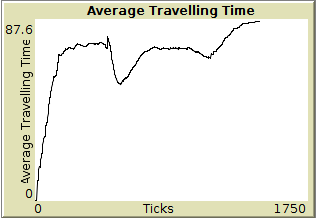
\includegraphics[width=\linewidth]{src/avg_tt5.png}
  \caption{Average travelling time in Day 5.}
  \label{fig:avg_tt5}
\end{minipage}
\end{figure}
